\definecolor{darkgreen}{rgb}{0,.6,0}
  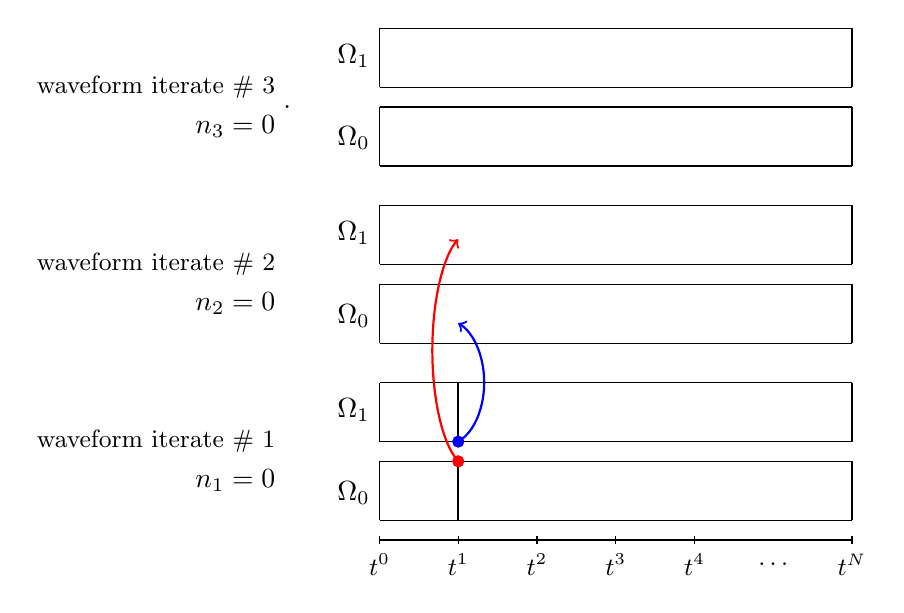
\begin{tikzpicture}[scale=1.0]

    \tikzstyle{dropline_style}=[densely dotted,thin]

    %\foreach \x/\xtext in {-1, -0.5/-\frac{1}{2}, 1}
    %\draw (\x cm,1pt) -- (\x cm,-1pt) node[anchor=north] {$\xtext$};

    \draw(-2,5) node[left] {.};
    \draw (-2.2, 0.75) node[left] {\small waveform iterate \# 1};
    \draw (-2.2, 3) node[left] {\small waveform iterate \# 2};
    \draw (-2.2, 5.25) node[left] {\small waveform iterate \# 3};

    \draw (-2.2, 0.25) node[left] {$n_1=0$};
    \draw (-2.2, 2.5) node[left] {$n_2=0$};
    \draw (-2.2, 4.75) node[left] {$n_3=0$};



    \def\a{-0.25}
    \def\b{0.5}
    \draw (-1,\a) -- (5,\a);
    \draw (5,\a) -- (5,\b);
    \draw (5,\b) -- (-1,\b);
    \draw (-1,\b) -- (-1,\a);

    \def\c{0.75}
    \def\d{1.5}
    \draw (-1,\c) -- (5,\c);
    \draw (5,\c) -- (5,\d);
    \draw (5,\d) -- (-1,\d);
    \draw (-1,\d) -- (-1,\c);

    \draw(-1,0.1) node[left] {$\Omega_0$};
    \draw(-1,1.15) node[left] {$\Omega_1$};

    \def\e{2}
    \def\f{2.75}
    \draw (-1,\e) -- (5,\e);
    \draw (5,\e) -- (5,\f);
    \draw (5,\f) -- (-1,\f);
    \draw (-1,\f) -- (-1,\e);

    \def\g{3}
    \def\h{3.75}
    \draw (-1,\g) -- (5,\g);
    \draw (5,\g) -- (5,\h);
    \draw (5,\h) -- (-1,\h);
    \draw (-1,\h) -- (-1,\g);

    \draw(-1,2.35) node[left] {$\Omega_0$};
    \draw(-1,3.4) node[left] {$\Omega_1$};

    \def\i{4.25}
    \def\j{5}
    \draw (-1,\i) -- (5,\i);
    \draw (5,\i) -- (5,\j);
    \draw (5,\j) -- (-1,\j);
    \draw (-1,\j) -- (-1,\i);

    \def\k{5.25}
    \def\l{6}
    \draw (-1,\k) -- (5,\k);
    \draw (5,\k) -- (5,\l);
    \draw (5,\l) -- (-1,\l);
    \draw (-1,\l) -- (-1,\k);

    \draw(-1,4.6) node[left] {$\Omega_0$};
    \draw(-1,5.65) node[left] {$\Omega_1$};


    % position of the time-line
    \def\y{-0.5}
    \draw [-] (-1,\y) -- (5,\y);

    \def\tick{0.05}
    \draw (-1,\y) ++(0,\tick) -- ++(0,-2*\tick) node[below] {\small $t^{0}$};
    \draw (0,\y) ++(0,\tick) -- ++(0,-2*\tick) node[below] {\small $t^{1}$};
    \draw (1,\y) ++(0,\tick) -- ++(0,-2*\tick) node[below] {\small $t^{2}$};
    \draw (2,\y) ++(0,\tick) -- ++(0,-2*\tick) node[below] {\small $t^{3}$};
    \draw (3,\y) ++(0,\tick) -- ++(0,-2*\tick) node[below] {\small $t^{4}$};
    \draw (4,\y)  node[below] {\small \phantom{t}$\ldots$\phantom{t}};  
    \draw (5,\y) ++(0,\tick) -- ++(0,-2*\tick) node[below] {\small $t^{N}$};
  
    % parameters for stencil diagrams
    \def\rad{0.12}
    \def\omr{0.88}   % 1-rad
    \def\intthick{0.068}   % thickness of integral bars

    %\draw [-latex,thick,blue] (-1,0.2) -- (0,0.2);
    %\draw [-latex,thick,blue] (-1,1.2) -- (0,1.2);

    \draw [-,thick,black] (0,\a) -- (0,\b);
    \draw [-,thick,black] (0,\c) -- (0,\d);

    %\draw (4,0.45)  node[below] {\small \phantom{t}$\ldots$\phantom{t}};  
    %\draw (4,1.45)  node[below] {\small \phantom{t}$\ldots$\phantom{t}};  
    
    % filled dots
    \foreach \xy in { (0,\b)}
    \filldraw [red] \xy circle (2pt);

    \foreach \xy in { (0,\c)}
    \filldraw [blue] \xy circle (2pt);


    \draw [->,thick,red] (0,0.5) arc (250:110:0.5 and 1.5);
    \draw [->,thick,blue] (0,0.75) arc (-70:70:0.5 and 0.8);

  \end{tikzpicture}
